\ifx\wholebook\relax \else
\documentclass[b5paper]{ctexart}
\usepackage[nomarginpar
  %, margin=.5in
]{geometry}

\addtolength{\oddsidemargin}{-0.05in}
\addtolength{\evensidemargin}{-0.05in}
\addtolength{\textwidth}{0.1in}
\usepackage[cn]{../../../prelude}

\setcounter{page}{1}

\begin{document}

\title{队列}

\author{刘新宇
\thanks{{\bfseries 刘新宇 } \newline
  Email: liuxinyu95@gmail.com \newline}
  }

\maketitle
\fi

\markboth{队列}{基本算法}

\ifx\wholebook\relax
\chapter{队列}
\numberwithin{Exercise}{chapter}
\fi

\section{简介}
\label{introduction}

队列提供了先进先出(FIFO)的机制。可以用多种方法实现队列,例如单向、双向链表,循环缓冲区等,Okasaki给出了16种不同的实现方法\cite{okasaki-book}。队列需要满足下面的两条基本要求:

\begin{enumerate}
\item 可以在常数时间内向末尾添加元素;
\item 可以在常数时间内从头部获取或删除元素。
\end{enumerate}

可以用双向链表直观地实现队列。我们略去这个简单的实现,而关注如何用其它基本数据结构,如列表、数组实现队列。

\section{列表实现}
\index{队列!单向链表实现}

我们可以用常数时间在列表头部插入、删除元素。但为了先进先出,我们只能在头部执行一种操作,而在尾部执行另一种操作。我们需要$O(n)$时间遍历整个列表以到达尾部,其中$n$是列表长度。这样就无法达到性能要求。为了解决这个问题,可以一个变量记录尾部位置。并用一个额外的节点$S$简化空队列的处理,如图\ref{fig:empty-list}所示。

\lstset{frame = single}
\begin{lstlisting}[language = Bourbaki]
data Node<K> {
  Key key
  Node next
}

data Queue {
  Node head, tail
}
\end{lstlisting}

\begin{figure}[htbp]
  \centering
  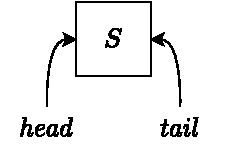
\includegraphics[scale=0.6]{img/empty-list}
  \caption{空队列,头、尾都指向$S$}
  \label{fig:empty-list}
\end{figure}

队列中最基本的两个操作是入队(Enqueue,或push、snoc、append、push back)和出队(Dequeue,或pop、pop front)。使用列表时,我们选择在头部加入元素、从尾部删除元素以简化实现。

\begin{algorithmic}[1]
\Function{Enqueue}{$Q, x$}
  \State $p \gets $ \Call{Node}{$x$}
  \State \Call{Next}{$p$} $\gets$ NIL
  \State \textproc{Next}(\Call{Tail}{$Q$}) $\gets p$
  \State \Call{Tail}{$Q$} $\gets p$
\EndFunction
\end{algorithmic}

队列至少有一个节点(空队列中有$S$节点),因此无需检查尾部是否为NIL。

\begin{algorithmic}[1]
\Function{Dequeue}{$Q$}
  \State $x \gets $ \Call{Head}{$Q$}
  \State \textproc{Next}(\Call{Head}{$Q$}) $\gets$ \Call{Next}{$x$}
  \If{$x = $ \Call{Tail}{$Q$}} \Comment{$Q$变为空}
    \State \Call{Tail}{$Q$} $\gets$ \Call{Head}{$Q$}
  \EndIf
  \State \Return \Call{Key}{$x$}
\EndFunction
\end{algorithmic}

$S$节点在所有其它节点的前面,\textproc{Head}实际返回$S$的下一个节点,如图\ref{fig:list-queue}所示。我们可以把这一实现扩展到并发环境。在头部和尾部各使用一把并发锁。$S$节点可以在队列空时避免死锁\cite{PODC96}、\cite{SutterDDJ}。

\begin{figure}[htbp]
  \centering
  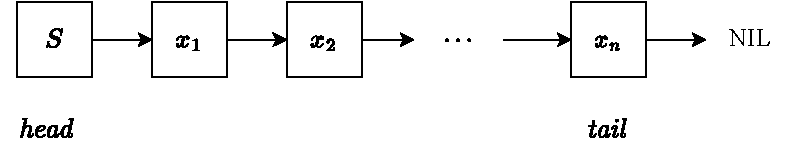
\includegraphics[scale=0.8]{img/slistq}
  \caption{带有$S$节点的列表}
  \label{fig:list-queue}
\end{figure}

\section{循环缓冲区}
\index{队列!循环缓冲区}

和列表相反,我们可以在常数时间将元素添加到数组末尾,但需要线性时间$O(n)$从头部删除。这是因为要将全部剩余元素依次向前移动。为了达到队列的性能要求,我们可以把数组的头尾连接起来,做成一个环,叫做循环缓冲区,如图如图\ref{fig:circular-buffer}、\ref{fig:circular-buffer-queue}所示。这样用数组的头部坐标head,队列长度count,和数组大小size,就可以完全表述队列。count等于0时队列为空,等于size时队列已满。我们还可以利用模运算简化入队、出队的实现。

\begin{figure}[htbp]
 \centering
 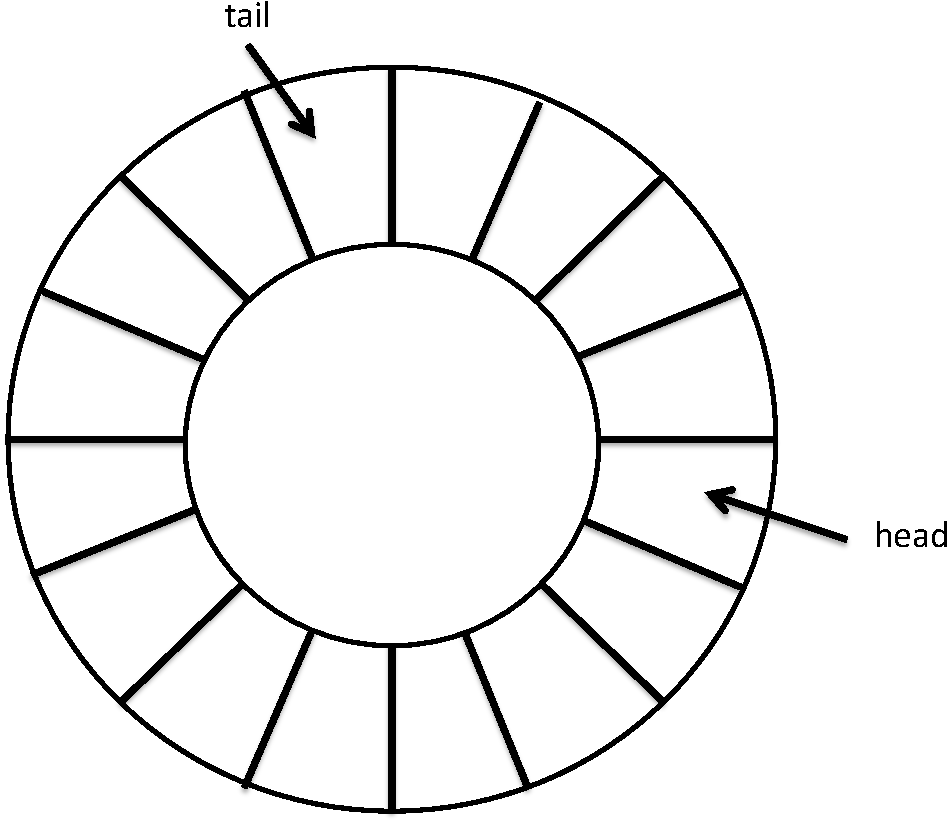
\includegraphics[scale=0.3]{img/ring-buffer}
 \caption{循环缓冲区}
 \label{fig:circular-buffer}
\end{figure}

\begin{figure}[htbp]
 \centering
 \subcaptionbox{连续加入多个元素。}{
 \begin{tikzpicture}[scale=0.8]
    \draw (0, 0) rectangle (1, 1) node (a0) [pos=.5] {a[0]}
          (1, 0) rectangle (2, 1) node [pos=.5] {a[1]}
          (2, 0) rectangle (3, 1) node [pos=.5] {...}
          (3, 0) rectangle (4, 1) node [pos=.5] (ai) {a[i]}
          (4, 0) rectangle (5, 1) node [pos=.5] {...}
          (5, 0) rectangle (6, 1) node (an) [pos=.5] {};
    \draw (0, 2) node (hd) {head}
          (3.5, 2) node (tl) {tail}
          (6, 2) node (bd) {边界};
    \draw[thick, ->] (hd) edge (a0)
                 (tl) edge (ai)
                 (bd) edge (an);
  \end{tikzpicture}}
 \subcaptionbox{从头部删除若干元素后,出现了空档。}{
  \begin{tikzpicture}[scale=0.8]
    \draw (0, 0) rectangle (1, 1)
          (1, 0) rectangle (2, 1) node [pos=.5] {...}
          (2, 0) rectangle (3, 1) node (aj) [pos=.5] {a[j]}
          (3, 0) rectangle (4, 1) node [pos=.5] {...}
          (4, 0) rectangle (5, 1) node (ai) [pos=.5] {a[i]}
          (5, 0) rectangle (6, 1) node [pos=.5] {...}
          (6, 0) rectangle (7, 1) node (an) [pos=.5] {};
    \draw (2, 2) node (hd) {head}
          (4.5, 2) node (tl) {tail}
          (7, 2) node (bd) {边界};
    \draw[thick, ->] (hd) edge (aj)
                 (tl) edge (ai)
                 (bd) edge (an);
  \end{tikzpicture}} \\
 \subcaptionbox{继续加入多个元素直到数组的边界。}{
   \begin{tikzpicture}[scale=0.8]
    \draw (0, 0) rectangle (1, 1)
          (1, 0) rectangle (2, 1) node [pos=.5] {...}
          (2, 0) rectangle (3, 1) node (aj) [pos=.5] {a[j]}
          (3, 0) rectangle (4, 1) node [pos=.5] {...}
          (4, 0) rectangle (5, 1) node (ai) [pos=.5] {a[i]};
    \draw (2, 2) node (hd) {head}
          (4.5, 2) node (tl) {tail}
          (6, 2) node (bd) {边界};
    \draw[thick, ->] (hd) edge (aj)
                 (tl) edge (ai)
                 (bd) edge [bend left] (ai);
  \end{tikzpicture}}
 \subcaptionbox{下一个元素加入到数组头部的第一个单元。}{
    \begin{tikzpicture}[scale=0.8]
    \draw (0, 0) rectangle (1, 1) node (a0) [pos=.5] {a[0]}
          (1, 0) rectangle (2, 1) node [pos=.5] {...}
          (2, 0) rectangle (3, 1) node (aj) [pos=.5] {a[j]}
          (3, 0) rectangle (4, 1) node [pos=.5] {...}
          (4, 0) rectangle (5, 1) node (an) [pos=.5] {};
    \draw (2.5, 2) node (hd) {head}
          (0, 2) node (tl) {tail}
          (6, 2) node (bd) {边界};
    \draw[thick, ->] (hd) edge (aj)
                 (tl) edge (a0)
                 (bd) edge (an);
  \end{tikzpicture}} \\
 \subcaptionbox{全部单元都保存了元素,队列已满。}{
   \begin{tikzpicture}[scale=0.8]
    \draw (0, 0) rectangle (1, 1) node [pos=.5] {a[0]}
          (1, 0) rectangle (2, 1) node [pos=.5] {a[1]}
          (2, 0) rectangle (3, 1) node [pos=.5] {...}
          (3, 0) rectangle (4, 1) node (a1j) [pos=.5] {a[j-1]}
          (4, 0) rectangle (5, 1) node (aj) [pos=.5] {a[j]}
          (5, 0) rectangle (6, 1) node [pos=.5] {...}
          (6, 0) rectangle (7, 1) node (an) [pos=.5] {};
    \draw (4.5, 2) node (hd) {head}
          (3, 2) node (tl) {tail}
          (7, 2) node (bd) {边界};
    \draw[thick, ->] (hd) edge (aj)
                 (tl) edge (a1j)
                 (bd) edge (an);
  \end{tikzpicture}}
 \caption{使用循环缓冲区实现队列} \label{fig:circular-buffer-queue}
\end{figure}

\begin{algorithmic}[1]
\Function{Enqueue}{$Q, x$}
  \If{not \Call{Full}{$Q$}}
    \State \Call{Count}{$Q$} $\gets$ \Call{Count}{$Q$} + 1
    \State tail $\gets $ (\Call{Head}{$Q$} + \Call{Count}{$Q$}) $\bmod$ \Call{Size}{$Q$}
    \State \Call{Buf}{$Q$}[tail] $\gets x$
  \EndIf
\EndFunction
\end{algorithmic}

\begin{algorithmic}[1]
\Function{Dequeue}{$Q$}
  \State $x \gets$ NIL
  \If{not \Call{Empty}{$Q$}}
    \State $h \gets$ \Call{Head}{$Q$}
    \State $x \gets$ \Call{Buf}{$Q$}[$h$]
    \State \Call{Head}{$Q$} $\gets $ (h + 1) $\bmod$ \Call{Size}{$Q$}
    \State \Call{Count}{$Q$} $\gets$ \Call{Count}{$Q$} - 1
  \EndIf
  \State \Return $x$
\EndFunction
\end{algorithmic}

\begin{Exercise}
循环缓冲区在初始化时规定了最大的容量,如果使用头、尾两个指针,而不用Count,如何检测队列是否为空?是否已满?(考虑两种情况:头部在尾部前面,和头部在尾部后面)。
\end{Exercise}

\section{双列表队列}
\index{队列!双列表队列}

列表的头部操作为常数时间,但尾部需要线性时间。我么可以把两个列表“尾对尾”连起来实现队列。形状类似一个马蹄形磁铁,如图\ref{fig:horseshoe-magnet}所示。两个列表分别叫做前(front)和后(rear)。队列记为$(f, r)$,空队列等于$([\ ], [\ ])$。我们把新元素加入$r$的头部,出队时,将元素从$f$的头部取走,性能都是常数时间。

\begin{figure}[htbp]
  \centering
  \subcaptionbox{马蹄形磁铁}{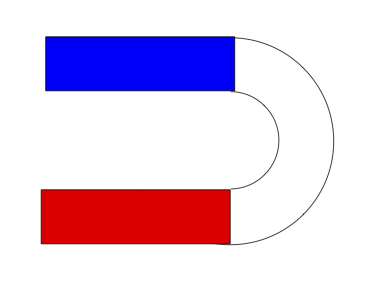
\includegraphics[scale=0.4]{img/horseshoe-magnet}} \\
  \subcaptionbox{“尾对尾”接在一起的列表}{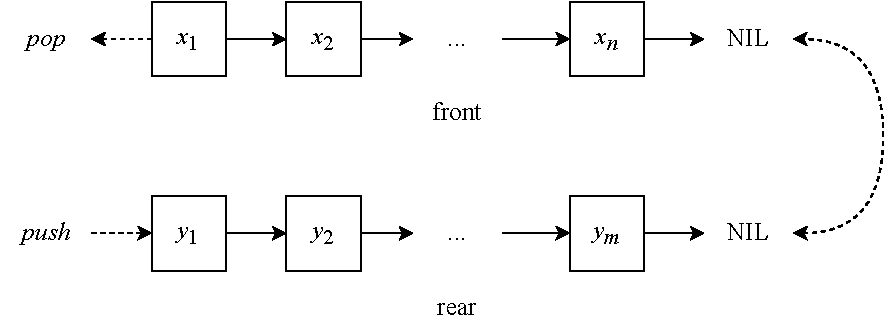
\includegraphics[scale=0.6]{img/paired-listq}}
  \caption{双列表队列}
  \label{fig:horseshoe-magnet}
\end{figure}

\be
\begin{cases}
push\ x\ (f, r) & = (f, x:r) \\
pop\ (x:f, r)   & = (f, r) \\
\end{cases}
\ee

经过一系列出队操作后,$f$可能为空,而$r$中还有元素。为了能继续出队,我们将$r$反转后替换掉$f$:$([\ ], r) \mapsto (reverse\ r, [\ ])$。为此每次出入队后,需要执行一次平衡检查和调整:

\be
\begin{array}{rcl}
\textit{balance}\ [\ ]\ r & = & (\textit{reverse}\ r, [\ ]) \\
\textit{balance}\ f\ r & = & (f, r) \\
\end{array}
\ee

一旦发生$r$的反转,则这次操作的性能下降为线性时间。尽管如此,整体的分摊复杂度是常数时间的。我们重新定义入队和出队为:

\be
\begin{cases}
push\ x\ (f, r) & = \textit{balance}\ f\ (x:r) \\
pop\ (x:f, r)   & = \textit{balance}\ f\ r \\
\end{cases}
\ee

\begin{Exercise}
为什么要在push时也要进行平衡检查和调整?
\end{Exercise}

\begin{Answer}
为什么要在push时也要进行平衡检查和调整?

考虑这样的情况:先$push\ a\ ([\ ], [\ ])$,然后再$pop$。
\end{Answer}

\section{双数组队列}
\index{队列!双数组队列}

和双列表相比,存在一个有趣的双数组对称实现。在某些老的编程语言中,例如旧版本的BASIC,只有数组可用,不能使用指针、或者结构等复合类型来定义链表。尽管可以使用一个额外的数组来记录索引,从而只用数组实现链表,但是还存在更简单的方法来队列,使得分摊性能为常数时间。

表\ref{tab:array-list-comp}比较了数组和链表,假设元素个数为$n$,各项操作的性能如下:

\begin{table}[htbp]
\centering
\begin{tabular}{l | c | r}
  \hline
  操作 & 数组 & 链表 \\
  \hline
  在头部加入 & $O(n)$ & $O(1)$ \\
  在尾部加入 & $O(1)$ & $O(n)$ \\
  在头部删除 & $O(n)$ & $O(1)$ \\
  在尾部删除 & $O(1)$ & $O(n)$ \\
  \hline
\end{tabular}
\caption{数组和链表各项操作的对比} \label{tab:array-list-comp}
\end{table}

可以看到,链表在头部的性能为常数时间,而在尾部为线性时间;而数组在尾部操作为常数时间(简单起见,假设空间足够,无需申请),但是在头部操作为线性时间。这是因为在头部插入时,需要将元素依次向后移动以预留出一个空挡,而删除时,需要将后继的元素依次向前移动以填补空挡(参见插入排序一章的介绍)。

上表给出了一个有趣的特性,我们可以利用它设计一个类似双列表的解决方法:将两个数组“头对头”连接起来,形成一个马蹄形的队列,如图\ref{fig:horseshoe-array}所示。

\begin{figure}[htbp]
  \centering
  \subcaptionbox{马蹄形磁铁}{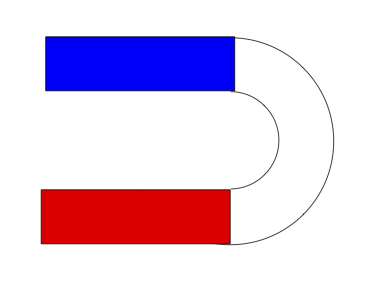
\includegraphics[scale=0.5]{img/horseshoe-magnet}}
  \subcaptionbox{将两个数组“头对头”连接起来}{\includegraphics[scale=0.5]{img/front-rear-array-queue}}
  \caption{使用front数组和rear数组实现的队列形如一个马蹄形磁铁} \label{fig:horseshoe-array}
\end{figure}

下面的Python例子程序定义了双数组队列\footnote{我们省略了旧式BASIC代码。在Python中,实际是使用了内置的list而不是array。也可参考本书附带的C/C++例子程序,它们使用内置的数组来实现队列。}。

\lstset{language=Python}
\begin{lstlisting}
class Queue:
    def __init__(self):
        self.front = []
        self.rear = []

def is_empty(q):
    return q.front == [] and q.rear == []
\end{lstlisting}

相应的入队操作\textproc{Push}()和出队操作\textproc{Pop}()都仅在数组的尾部执行。

\begin{algorithmic}
\Function{Push}{$Q, x$}
  \State \textproc{Append}(\Call{Rear}{$Q$}, $x$)
\EndFunction
\end{algorithmic}

其中过程\textproc{Append}()将元素$x$加入到数组的尾部,并进行必要的内存申请。有多种内存处理策略,除了重新申请更大的内存,然后复制元素外,还可以设置内存上限,并在用满后报错。

出队操作算法的定义如下:

\begin{algorithmic}
\Function{Pop}{$Q$}
  \If{\Call{Front}{$Q$} $= \phi$}
    \State \Call{Front}{$Q$} $\gets$ \textproc{Reverse}(\Call{Rear}{$Q$})
    \State \Call{Rear}{$Q$} $\gets \phi$
  \EndIf
  \State $n \gets$ \textproc{Length}(\Call{Front}{$Q$})
  \State $x \gets$ \Call{Front}{$Q$}[n]
  \State \textproc{Length}(\Call{Front}{$Q$}) $\gets n - 1$
  \State \Return $x$
\EndFunction
\end{algorithmic}

简单起见,在删除元素后,我们并未缩小数组的尺寸。可以通过检查数组的长度是否为0来判断front数组是否为空。这里跳过了这些细节。

下面的Python例子程序实现了入队和出队操作。

\begin{lstlisting}
def push(q, x):
    q.rear.append(x)

def pop(q):
    if q.front == []:
        q.rear.reverse()
        (q.front, q.rear) = (q.rear, [])
    return q.front.pop()
\end{lstlisting}

和paried-list队列类似,由于反转数组也是线性时间的,这一实现的分摊性能为常数时间$O(1)$。

\begin{Exercise}
\begin{itemize}
\item 证明双列表队列的分摊性能为常数时间$O(1)$。
\item 证明双数组队列的分摊性能为常数时间$O(1)$。
\end{itemize}
\end{Exercise}

% ================================================================
%                 Balanced Queue
% ================================================================
\section{平衡队列}
\index{队列!平衡队列}

虽然双列表队列的入队和出队操作的分摊复杂度为常数时间$O(1)$,但是在最坏情况下的性能很差。例如front列表中只有一个元素,然后我们将$n$个元素连续加入队列,这里$n$是一个很大的整数。此时执行一次出队操作就会进入最坏情况。

根据规则,全部$n$个元素都加入了rear列表。执行一次弹出操作后,front列表变为空。于是开始反转rear列表,这一操作是线性时间$O(n)$的,和rear列表的长度成比例。某些场合下,当$n$很大时,这一时间消耗太大,无法满足要求。

造成这一最坏情况的原因是由于front和rear列表极不平衡。我们可以修改队列的设计来改进平衡性。例如加入一条平衡限制:

\be
  | R | \leq | F |
\label{eq:balance-invariant}
\ee

其中$R = Rear(Q)$,$F = Front(Q)$分别是队列中的前后两个列表。记号$|L|$表示列表$L$的长度。这一条件保证了rear列表的长度不大于front列表。当条件不满足时,就执行反转操作。

使用这一限制条件,需要频繁获取列表的长度。由于列表本质上是单向链表,因此需要线性时间来得到长度。我们可以将列表的长度缓存起来,并在增减元素时更新长度。这样就可以在常数时间获得列表长度。

下面的Haskell例子代码在双列表队列的基础上增加了长度缓存信息。

\lstset{language=Haskell}
\begin{lstlisting}[style=Haskell]
data BalanceQueue a = BQ [a] Int [a] Int
\end{lstlisting}

只要保持式(\ref{eq:balance-invariant})一直得到满足,就可以通过检查front列表的长度来判断队列是否为空:

\be
  F = \phi \Leftrightarrow |F| = 0
\ee

本节余下的部分中,我们一律认为可以在常数时间内获得列表$L$的长度$|L|$。

入队和出队操作基本和以前一样,我们需要额外传入列表的长度信息,检查平衡条件,如有必要就执行反转操作。

\be
  push(Q, x) = balance(F, |F|, \{ x \} \cup R, |R| + 1)
\ee

\be
  pop(Q) = balance(tail(F), |F|-1, R, |R|)
\ee

其中函数$balance()$定义如下:

\be
  balance(F, |F|, R, |R|) = \left \{
  \begin{array}
  {r@{\quad:\quad}l}
  Queue(F, |F|, R, |R|) & |R| \leq |F| \\
  Queue(F \cup reverse(R), |F| + |R|, \phi, 0) & otherwise
  \end{array}
\right .
\ee

这里函数$Queue()$接受四个参数:front列表和缓存的长度;rear列表和长度。这些信息用以构造一个双列表队列。

下面的Haskell例子程序实现了平衡双列表队列。程序使用了Haskell的类型系统来保证实现符合抽象队列的定义。

\lstset{language=Haskell}
\begin{lstlisting}[style=Haskell]
instance Queue BalanceQueue where
    empty = BQ [] 0 [] 0

    isEmpty (BQ _ lenf _ _) = lenf == 0

    -- Amortized O(1) time push
    push (BQ f lenf r lenr) x = balance f lenf (x:r) (lenr + 1)

    -- Amortized O(1) time pop
    pop (BQ (_:f) lenf r lenr) = balance f (lenf - 1) r lenr

    front (BQ (x:_) _ _ _) = x

balance f lenf r lenr
    | lenr <= lenf = BQ f lenf r lenr
    | otherwise = BQ (f ++ (reverse r)) (lenf + lenr) [] 0
\end{lstlisting}

\begin{Exercise}
选择一门命令式语言,实现平衡双数组队列。
\end{Exercise}

% ================================================================
%                 Realtime Queue
% ================================================================
\section{实时队列}
\index{队列!实时队列}

改善平衡性后虽然可以避免最差情况,但是反转rear列表的的性能仍然是$O(n)$的,其中$n = |R|$。尽管分摊性能为常数时间,但如果rear列表很长,某次操作的性能仍然会很差。在某些实时系统中,我们必须保证在最坏情况下的性能也达到要求。

根据前面的分析,计算的瓶颈在$ F \cup reverse(R)$,当$|R| > |F|$时会发生这一操作。考虑$|F|$和$|R|$都是整数,发生这一操作时,我们有:

\be
  |R| = |F| + 1
\ee

$F$和$reverse(R)$的结果都是单向链表,连接它们耗时$O(|F|)$,此外还需要$O(|R|)$时间反转rear列表,因此总时间为$O(n)$,其中$n = |F| + |R|$。也就是说,和队列中的元素个数成正比。

为了实现实时队列,我们不能一次性计算$ F \cup reverse(R)$。解决策略是将这一耗时的计算分派到各次入队和出队操作中去。这样虽然单次的入队和出队需要做的事情多了,但是可以避免最坏情况下性能退化为线性时间。

\subsection{逐步反转}
\index{队列!逐步反转}

我们首先分析一下典型的函数式反转算法。

\be
  reverse(X) = \left \{
  \begin{array}
  {r@{\quad:\quad}l}
  \phi & X = \phi \\
  reverse(X') \cup \{ x_1 \} & otherwise
  \end{array}
\right .
\ee

其中$X' = tail(X) = \{ x_2, x_3, ...\}$。

若列表为空,则反转结果也是一个空列表。否则,我们取出第一个元素$x_1$,将剩余元素$\{x_2, x_3, ..., x_n \}$反转为$\{x_n, x_{n-1}, .., x_3, x_2 \}$,然后再将$x_1$追加到末尾。

但是,这一算法的性能不佳,追加元素到末尾用时和列表长度成正比。因此这一反转操作的性能为$O(n^2)$。

另外一种实现方式是使用\underline{尾递归}:

\be
  reverse(X) = reverse'(X, \phi)
\ee

其中

\be
 reverse'(X, A) = \left \{
  \begin{array}
  {r@{\quad:\quad}l}
  A & X = \phi \\
  reverse'(X', \{ x_1 \} \cup A) & otherwise
  \end{array}
\right .
\ee

我们称$A$为\underline{累积器}(accumulator),它不断累积中间结果。任何时候,当调用$reverse'(X, A)$时,$X$包含尚未反转的元素,$A$包含迄今为止反转完的元素。当第$i$次调用$reverse'()$时,$X$和$A$分别包含如下内容:

\[
  \begin{array}{r@{\quad}l}
  X = \{x_i, x_{i+1}, ..., x_n \} & A = \{ x_{i-1}, x_{i-2}, ... x_1 \}
  \end{array}
\]

每次递归,如果不是边界情况,我们用常数时间从$X$取出第一个元素;然后将其链结到$A$的前面,这一步同样仅耗时常数时间$O(1)$。同样的操作重复$n$次,因此这一反转算法是线性时间$O(n)$的。

尾递归\cite{wiki-tail-call}\cite {recursion}算法可以很容易从一次性计算改为逐步计算。整体过程相当于一系列的状态转换。我们定义一个状态机,包含两种状态:反转状态$S_r$表示正在进行反转(未完成);完成状态$S_f$表示反转已经结束(完成)。下面的Haskell例子程序将状态定义为类型。

\lstset{language=Haskell}
\begin{lstlisting}[style=Haskell]
data State a = | Reverse [a] [a]
               | Done [a]
\end{lstlisting}

使用这两种状态,我们可以调度(slow-down)函数$reverse'(X, A)$的计算:

\be
  step(S, X, A) = \left \{
  \begin{array}
  {r@{\quad:\quad}l}
  (S_f, A) & S = S_r \land X = \phi \\
  (S_r, X', \{ x_1 \} \cup A) & S = S_r \land X \neq \phi \\
  \end{array}
\right .
\ee

每一步,我们先检查当前的状态,如果状态为$S_r$(反转中),但是$X$中已没有剩余元素需要反转,就将状态变换为完成$S_f$;否则,我们取出$X$中的第一个元素,将其链结到$A$的前面,接下来与之前不同,我们不再进行递归调用,这一步计算到此结束。当前的状态,以及反转的中间步骤结果$X$和$A$被保存下来,我们可以在以后的任何时候使用这些内容,再调用$step$函数继续反转。

下面是逐步反转的一个例子:

\[
\begin{array}{lcl}
step(S_r, \text{``hello''}, \phi) & = & (S_r, \text{``ello''}, \text{``h''}) \\
step(S_r, \text{``ello''}, \text{``h''}) & = & (S_r, \text{``llo''}, \text{``eh''}) \\
... & & \\
step(S_r, \text{``o''}, \text{``lleh''}) & = & (S_r, \phi, \text{``olleh''}) \\
step(S_r, \phi, \text{``olleh''}) & = & (S_f, \text{``olleh''})
\end{array}
\]

下面的Haskell代码描述了同样的例子:

\lstset{language=Haskell}
\begin{lstlisting}[style=Haskell]
step $ Reverse "hello" [] = Reverse "ello" "h"
step $ Reverse "ello" "h" = Reverse "llo" "eh"
...
step $ Reverse "o" "lleh" = Reverse [] "olleh"
step $ Reverse [] "olleh" = Done "olleh"
\end{lstlisting}

现在我们可以将反转计算逐步分散到入队和出队操作中。但是这仅解决了一半问题。我们需要逐步分解$ F \cup reverse(R)$计算。因此接下来需要调度(slow-down)列表的连接操作$F \cup ...$。连接操作的复杂度为$O(|F|)$。同样,我们的目标是将它分散到入队和出队操作中去。

\subsection{逐步连接}
\index{队列!逐步连接}

实现列表的逐步连接要比逐步反转难度更大。我们可以利用逐步反转的结果。这里有一个小技巧:为了实现$X \cup Y$,我们可以先将$X$反转为$\overleftarrow{X}$,然后逐一将$\overleftarrow{X}$中的元素取出,放到$Y$的前面。这和我们前面实现的$reverse'$类似。

\be
  \begin{array}{rcl}
    X \cup Y & \equiv & reverse(reverse(X)) \cup Y \\
             & \equiv & reverse'(reverse(X), \phi) \cup Y \\
             & \equiv & reverse'(reverse(X), Y) \\
             & \equiv & reverse'(\overleftarrow{X}, Y)
  \end{array}
\ee

这一事实表明,我们可以增加另一个状态来控制$step()$函数,在$R$反转后,逐步操作$\overleftarrow{F}$实现连接。

整个操作被分解为两个阶段:

\begin{enumerate}
\item 同时反转$F$和$R$,逐步得到$\overleftarrow{F} = reverse(F)$和$\overleftarrow{R} = reverse(R)$;
\item 逐步从$\overleftarrow{F}$取出元素,链接到$\overleftarrow{R}$前面。
\end{enumerate}

为此我们定义三种状态:$S_r$代表反转;$S_c$代表连接;$S_f$代表完成。

下面的Haskell例子程序定义了这三种状态。

\lstset{language=Haskell}
\begin{lstlisting}[style=Haskell]
data State a = Reverse [a] [a] [a] [a]
             | Concat [a] [a]
             | Done [a]
\end{lstlisting}

由于我们同时反转$F$和$R$,因此反转状态变量带有一对列表和一对累积器。

状态转换按照两个阶段策略进行定义。记$F = \{ f_1, f_2, ... \}$、$F' = tail(F) = \{f_2, f_3, ... \}$、
$R = \{ r_1, r_2, ... \}$、$R' = tail(R) = \{ r_2, r_3, ... \}$。一个状态$\mathcal{S}$包含它的类型$S$,可以是$S_r$、$S_c$和$S_f$的一种。同时状态$\mathcal{S}$中还包含必要的参数,如$F$、$\overleftarrow{F}$、$X$、$A$等作为中间结果。状态不同,包含的参数也有所不同。

\be
  next(\mathcal{S}) = \left \{
  \begin{array}
  {r@{\quad:\quad}l}
  (S_r, F', \{ f_1 \} \cup \overleftarrow{F}, R', \{ r_1 \} \cup \overleftarrow{R}) & S = S_r \land F \neq \phi \land R \neq \phi \\
  (S_c, \overleftarrow{F}, \{ r_1 \} \cup \overleftarrow{R}) & S = S_r \land F = \phi \land R = \{ r_1 \} \\
  (S_f, A) & S = S_c \land X = \phi \\
  (S_c, X', \{ x_1 \} \cup A) & S = S_c \land X \neq \phi
  \end{array}
\right .
\ee

相应的Haskell程序如下:

\lstset{language=Haskell}
\begin{lstlisting}[style=Haskell]
next (Reverse n (x:f) f' (y:r) r') = Reverse (n + 1) f (x:f') r (y:r')
next (Reverse n [] f' [y] r') = Concat n f' (y:r')
next (Concat 0 _ acc) = Done acc
next (Concat n (x:f') acc) = Concat (n - 1) f' (x:acc)
\end{lstlisting}

接下来我们需要将这些递进的步骤分配到每个出队和入队操作中以实现一个实时$O(1)$的纯函数式队列。

\subsection{汇总}

在给出最终的实现前,我们先来分析一下为了计算$F \cup reverse(R)$,总共需要多少递进步骤。根据平衡队列的条件,有$|R| = |F| + 1$。记$m = |F|$。

由于某次出队或入队操作造成队列不平衡时,我们开始逐步计算$F \cup reverse(R)$。总共需要$m+1$步来反转$R$,我们同时在这些步骤内完成了对$F$的反转。此后,我们需要再用$m+1$步来进行连接操作。因此总共花费了$2m+2$步。

最直观的想法是在每一个出队和入队操作中分配一个递进步骤。但是我们需要回答一个关键问题:在我们完成$2m+2$步操作之前,队列有没有可能由于接下来的一系列入队和出队操作,再次变得不平衡?

关于这一问题有两个事实,一个是好消息,一个是坏消息。

我们先看好消息。很幸运,在我们花费$2m+2$步操作计算$F \cup reverse(R)$完成之前,连续的入队操作不可能再次使得队列变得不平衡。因为一旦开始恢复平衡的处理,经过$2m+2$步后,我们就得到了一个新的front列表$F' = F \cup reverse(R)$。而下一次队列变得不平衡时,我们有:

\be
  \begin{array}{rcl}
  |R'| & = & |F'| + 1 \\
       & = & |F| + |R| + 1 \\
       & = & 2m + 2
  \end{array}
\ee

也就是说,从上次队列不平衡的时刻算起,即使我们不断持续将新元素入队,以最快的速度再次使得队列不平衡时,$2m+2$步计算恰好已经完成了。此时新的front列表被计算出来。我们可以安全地继续计算$F' \cup reverse(R')$。多亏了前面给出的平衡不变特性(invariant),帮助我们保证了这一点。

但是还有一个坏消息。在$2m+2$步计算完成前,出队操作可能随时发生。这会产生一个尴尬的情况:我们需要从front列表取出元素,但是新的front列表$F' = F \cup reverse(R)$尚未计算好。此时没有一个可用的front列表。

一种解决方法是在第一阶段计算$reverse(F)$时,另外保存一份此前的front列表$F$。这样即使连续进行$m$次出队操作,我们仍然是安全的。表(\ref{tab:pop-before-m})给出了第一阶段逐步计算(同时反转$F$和$R$)的某个时刻队列的样子\footnote{有人会产生疑问,通常复制一个列表需要花费和列表长度成比例的线性时间。这样整个方案就有问题了。实际上,这一线性时间的列表复制根本不会发生。因为在纯函数式的环境下,出队或反转并不“修改”front列表。但是,如果尝试用双数组实现一个对称解,并且就地修改数组,这一问题就会产生影响。为此,我们需要实现某种lazy复制,真正的复制操作并不立即发生,而是在每次反转的递进步骤中一步复制一个元素。具体的实现留给读者作为练习。}。

\begin{table}[htbp]
\centering
\begin{tabular}{l l l}
  保存的front列表 & 进行中的计算 & 新的rear列表 \\
  \hline
  $\{ f_i, f_{i+1}, ..., f_M \}$ & $(S_r, \tilde{F}, ..., \tilde{R}, ...)$ & $ \{ ... \}$ \\
  前$i-1$个元素已出队 & $\overleftarrow{F}$和$\overleftarrow{R}$的中间结果 & 包含新入队的元素
\end{tabular}
\caption{前$m$步完成之前的队列中间状态}
\label{tab:pop-before-m}
\end{table}

经过$m$次出队操作,$F$的副本已经用光。我们此时刚刚开始进逐步连接的计算阶段。此时如果继续进行出队操作会怎样?

事实上,由于$F$的副本被用光(变成了$\phi$),我们无需再进行连接操作了。这是因为$F \cup \overleftarrow{R} = \phi \cup \overleftarrow{R} = \overleftarrow{R}$。

这一点告诉我们,在进行连接操作时,我们只需要将$F$中尚未出队的元素连接起来。因为元素从$F$的头部逐一出队,我们可以使用一个计数器(counter)来记录$F$中剩余元素的个数。当开始计算$F \cup reverse(R)$时,计数器为0,每次反转$F$中的一个元素时,就将计数器加一,表示将来我们需要连接这个元素;每次出队操作,就将计数器减一,表示我们将来可以少连接一个元素。显然在连接操作的每步中,我们也需要递减计数器。当且仅当计数器为0的时候,我们无需继续进行连接操作。

根据以上的分析,我们可以给出纯函数式的实时队列的完整实现了。为了简化状态转换,我们可以增加一个空闲状态$S_0$。下面的Haskell例子程序给出了这一修改过的状态定义。

\lstset{language=Haskell}
\begin{lstlisting}[style=Haskell]
data State a = Empty
             | Reverse Int [a] [a] [a] [a] -- n, f', acc\_f' r, acc\_r
             | Append Int [a] [a]          -- n, rev\_f', acc
             | Done [a] -- result: f ++ reverse r
\end{lstlisting}

队列的数据结构分为三个部分:front列表(带有长度信息);正在计算中的$F \cup reverse(R)$的中间状态;和rear列表(带有长度信息)。

下面的Haskell例子程序定义了实时队列的数据结构。

\lstset{language=Haskell}
\begin{lstlisting}[style=Haskell]
data RealtimeQueue a = RTQ [a] Int (State a) [a] Int
\end{lstlisting}

空队列包含空的front和rear列表,以及一个空闲状态$S_0$,记为$Queue(\phi, 0, S_0, \phi, 0)$。根据平衡invariant的定义,我们可以通过检查$|F|=0$与否来判断一个队列是否为空。入队和出队操作修改如下:

\be
  push(Q, x) = balance(F, |F|, \mathcal{S}, \{ x \} \cup R, |R|+1)
\ee

\be
  pop(Q) = balance(F', |F|-1, abort(\mathcal{S}), R, |R|)
\ee

最大的变化在于$abort()$函数。根据前面的分析,在出队时我们递减计数器,这样将来可以少连接一个元素。我们将其定义为撤销操作。我们稍后介绍它的具体实现。

相应的Haskell出队和入队操作可以由下面的例子程序给出。

\lstset{language=Haskell}
\begin{lstlisting}[style=Haskell]
push (RTQ f lenf s r lenr) x = balance f lenf s (x:r) (lenr + 1)
pop (RTQ (_:f) lenf s r lenr) = balance f (lenf - 1) (abort s) r lenr
\end{lstlisting}

函数$balance()$首先检查平衡invariant,如果违反了,我们需要启动$F \cup reverse(R)$的逐步计算来恢复平衡;否则,我们仅仅执行一步尚未完成的递进计算。

\be
  balance(F, |F|, \mathcal{S}, R, |R|) = \left \{
  \begin{array}
  {r@{\quad:\quad}l}
  step(F, |F|, \mathcal{S}, R, |R|) & |R| \leq |F| \\
  step(F, |F| + |R|, (S_r, 0, F, \phi, R, \phi) \phi, 0) & otherwise
  \end{array}
\right .
\ee

相应的Haskell例子程序如下:

\lstset{language=Haskell}
\begin{lstlisting}[style=Haskell]
balance f lenf s r lenr
    | lenr <= lenf =  step f lenf s r lenr
    | otherwise = step f (lenf + lenr) (Reverse 0 f [] r []) [] 0
\end{lstlisting}

函数$step()$将状态机转换到下一个状态,全部递进计算结束后,状态转换到空闲状态$S_0$。

\be
  step(F, |F|, \mathcal{S}, R, |R|) = \left \{
  \begin{array}
  {r@{\quad:\quad}l}
  Queue(F', |F|, S_0, R, |R|) &  S' = S_f \\
  Queue(F, |F|, \mathcal{S}', R, |R|) & otherwise
  \end{array}
  \right .
\ee

其中,$\mathcal{S}' = next(\mathcal{S})$,是下一个转换到的状态;$F' = F \cup reverse(R)$是递进计算出的新front列表。真正的状态转换函数$next()$的实现如下。和前面的定义不同,我们增加了一个计数器$n$来记录还剩余多少个元素需要连接。

\be
  next(\mathcal{S}) = \left \{
  \begin{array}
  {r@{\quad:\quad}l}
  (S_r, n+1, F', \{ f_1 \} \cup \overleftarrow{F}, R', \{ r_1 \} \cup \overleftarrow{R}) &
      S = S_r \land F \neq \phi \\
  (S_c, n, \overleftarrow{F}, \{ r_1 \} \cup \overleftarrow{R}) &
      S = S_r \land F = \phi \\
  (S_f, A) & S = S_c \land n = 0 \\
  (S_c, n-1, X', \{ x_1 \} \cup A) & S = S_c \land n \neq 0 \\
  \mathcal{S} & otherwise
  \end{array}
\right .
\ee

相应的Haskell例子程序如下:

\lstset{language=Haskell}
\begin{lstlisting}[style=Haskell]
next (Reverse n (x:f) f' (y:r) r') = Reverse (n+1) f (x:f') r (y:r')
next (Reverse n [] f' [y] r') = Concat n f' (y:r')
next (Concat 0 _ acc) = Done acc
next (Concat n (x:f') acc) = Concat (n-1) f' (x:acc)
next s = s
\end{lstlisting}

函数$abort()$用于指示状态机,由于发生了出队操作,可以少连接一个元素。

\be
  abort(\mathcal{S}) = \left \{
  \begin{array}
  {r@{\quad:\quad}l}
  (S_f, A') & S = S_c \land n = 0 \\
  (S_c, n-1, X' A) & S = S_c \land n \neq 0 \\
  (S_r, n-1, F, \overleftarrow{F}, R, \overleftarrow{R}) & S = S_r \\
  \mathcal{S} & otherwise
  \end{array}
\right .
\ee

注意当$n = 0$的时候,我们实际上撤销了上一个链接元素的操作,因此返回$A'$而不是$A$作为结果(作为练习,我们请读者来回答这样做的原因)。

下面的Haskell例子程序实现了abort函数。

\lstset{language=Haskell}
\begin{lstlisting}[style=Haskell]
abort (Concat 0 _ (_:acc)) = Done acc      -- 注意:我们回滚(rollback)了一个元素
abort (Concat n f' acc) = Concat (n-1) f' acc
abort (Reverse n f f' r r') = Reverse (n-1) f f' r r'
abort s = s
\end{lstlisting}

我们已经接近最终的结果了。但是仍有一个隐藏的问题必须解决:如果将一个元素$x$放入一个空队列,结果会是:

\[
  Queue(\phi, 1, (S_c, 0, \phi, \{ x \}), \phi, 0)
\]

若此时立即进行出队操作,就会发生错误!虽然上一次$F \cup reverse(R)$的计算已经结束,但是front列表却为空。这是因为还需要额外一步才能从状态$(S_c, 0, \phi, A)$转换到$(S_f, A)$。因此需要进一步调整函数$step()$中的$\mathcal{S}'$如下:

\be
  \mathcal{S}' = \left \{
  \begin{array}
  {r@{\quad:\quad}l}
  next(next(\mathcal{S})) & F = \phi \\
  next(\mathcal{S}) & otherwise
  \end{array}
\right .
\ee

下面的Haskell例子程序体现了这一修改:

\lstset{language=Haskell}
\begin{lstlisting}[style=Haskell]
step f lenf s r lenr =
    case s' of
      Done f' -> RTQ f' lenf Empty r lenr
      s' -> RTQ f lenf s' r lenr
    where s' = if null f then next $ next s else next s
\end{lstlisting} %$

注意这一算法和Chris Okasaki在\cite{okasaki-book}给出的有所不同。Okasaki的算法每次出队、入队执行两步递进计算,而本章中的算法每次只执行一次。因此计算性能的分布更加均匀。

\begin{Exercise}
\begin{itemize}
\item 在$abort()$函数中,当$n = 0$时,为什么需要回滚一个元素?

\item 考虑实时队列的对称实现。选择一门命令式语言,用双数组实现实时队列。

\item 在脚注中,我们提到,使用就地修改的双数组来实现实时队列时,当开始递进计算反转时,不能一次性复制数组,否则就会将性能降低到线性时间复杂度。请实现一个惰性复制(lazy copy),使得每步反转时我们仅复制一个元素。

\end{itemize}
\end{Exercise}


% ================================================================
%                 Lazy Real-time queue
% ================================================================
\section{惰性实时队列}
\index{队列!惰性实时队列}

实现实时队列的关键在于将耗时的$F \cup reverse(R)$计算分解。惰性求值对于这类问题很有帮助。本节中,我们通过惰性求值来寻找更加简洁的方法。

假设存在一个函数$rotate()$可以逐步计算$F \cup reverse(R)$。也就是说,使用一个累积器$A$,下面的两个函数等价

\be
  rotate(X, Y, A) \equiv X \cup reverse(Y) \cup A
  \label{eq:rot-def}
\ee

其中,我们将$X$初始化为front列表$F$,$Y$初始化为rear列表$R$,$A$初始化为空$\phi$。

开始进行轮转(rotate)的条件和前面一样,即$|F| + 1 = |R|$。在轮转过程中,我们始终保持$|X| + 1 = |Y|$作为一个不变式成立。

下面我们来推导轮转的实现,显然,最简单的情况如下:

\be
  rotate(\phi, \{ y_1 \}, A) = \{ y_1 \} \cup A
\ee

记$X = \{ x_1, x_2, ... \}$、$Y = \{ y_1, y_2, ...\}$;而$X' = \{ x_2, x_3, ...  \}$、$Y' = \{ y_2, y_3, ...\}$是$X$和$Y$除去第一个元素以外的剩余元素。递归情况可以推导如下:

\be
  \begin{array}{rcll}
  rotate( X, Y, A ) & \equiv & X \cup reverse(Y) \cup A & \mbox{根据定义(}\ref{eq:rot-def} \mbox{的定义} \\
  & \equiv & \{ x_1 \} \cup (X' \cup reverse(Y) \cup A) & \cup \mbox{操作的结合性} \\
  & \equiv & \{ x_1 \} \cup (X' \cup reverse(Y') \cup (\{ y_1 \} \cup A)) & \mbox{reverse的性质和}  \cup \mbox{的结合性} \\
  & \equiv & \{ x_1 \} \cup rotate(X', Y', \{ y_1 \} \cup A) & \mbox{根据定义(} \ref{eq:rot-def} \mbox{)}
  \end{array}
\ee

归纳上面的两种情况,可以得到最终的轮转算法。

\be
rotate(X, Y, A) = \left \{
  \begin{array}
  {r@{\quad:\quad}l}
  \{ y_1 \} \cup A & X = \phi \\
  \{ x_1 \} \cup rotate(X', Y', \{ y_1 \} \cup A) & otherwise
  \end{array}
\right .
\ee

如果我们惰性执行$\cup$操作,而不是立即进行链接,也就是说,当出队和入队时才执行$\cup$,就可以将$rotate$计算自然分摊到出、入队中。

根据这一思路,我们修改双列表队列的定义,将front列表变成一个惰性列表,然后将它放入一个流(stream)中\cite{SICP}。当某个出、入队操作,造成队列的平衡被破坏,此时有$|F| + 1 = |R|$,为了恢复平衡,我们开始进行惰性轮转计算。这一惰性计算被作为新的front列表$F'$,而新的rear列表为空$\phi$。我们同时维护一个$F'$的副本作为流。

此后,每当进行出、入队操作,我们就强制流执行一个$\cup$操作。这样流就向前执行一步$ \{ x \} \cup F''$,其中$F'' = tail(F')$。我们丢掉$x$,然后用$F''$替换$F'$作为新的流。

当全部流被计算完毕,就可以开始计算另一个轮转。

为了更好地描述这一思路,我们使用Scheme/Lisp给出例子程序。这样可以明确地控制惰性计算。

\lstset{language=Lisp}
\begin{lstlisting}
(define (cons-stream a b) (cons a (delay b)))

(define stream-car car)

(define (stream-cdr s) (cdr (force s)))
\end{lstlisting}

函数\texttt{cons-stream}从一个元素$x$和列表$L$构造一个惰性列表。它并不对列表$L$求值,求值被推迟到\texttt{stream-cdr}中进行。延迟求值可以通过lambda演算来实现\cite{SICP}。

下面的例子程序给出了惰性双列表队列的定义。

\lstset{language=Lisp}
\begin{lstlisting}
(define (make-queue f r s)
  (list f r s))

(define (front-lst q) (car q))

(define (rear-lst q) (cadr q))

(define (rots q) (caddr q))
\end{lstlisting}

一个队列包含三个部分:一个front列表,一个rear列表和一个代表计算$F \cup reverse(R)$的流。对于空队列,这三个部分全部是null。

\begin{lstlisting}
(define empty (make-queue '() '() '()))
\end{lstlisting}

注意,其中的front列表实际上是一个惰性流,因此需要使用流相关的操作。例如下面的函数通过检查front流来判断队列是否为空。

\begin{lstlisting}
(define (empty? q) (stream-null? (front-lst q)))
\end{lstlisting}

入队函数和上一节所介绍的基本相同。我们将新加入的元素放到rear列表前面,然后检查平衡条件,如果不满足就需要恢复平衡。

\be
push(Q, x) = balance(\mathcal{F}, \{ x \} \cup R, \mathcal{R}_s)
\ee

其中$\mathcal{F}$是表示front列表的惰性流;$\mathcal{R}_s$是表示轮转计算的流。相应的Scheme/Lisp例子程序如下:

\begin{lstlisting}
(define (push q x)
  (balance (front-lst q) (cons x (rear q)) (rots q)))
\end{lstlisting}

出队操作和此前相比有一些不同,由于front列表实际是一个惰性流,我们需要进行强制求值,其余部分保持不变。

\be
pop(Q) = balance(\mathcal{F}', R, \mathcal{R}_s)
\ee

其中$\mathcal{F}'$强制对$\mathcal{F}$进行一次求值,相应的Scheme/Lisp例子程序如下:

\begin{lstlisting}
(define (pop q)
  (balance (stream-cdr (front-lst q)) (rear q) (rots q)))
\end{lstlisting}

为了节省篇幅,我们省略了错误处理(例如对空队列进行出队操作的错误等)。

通过从front流中提取元素可以获得队列的头部元素。

\begin{lstlisting}
(define (front q) (stream-car (front-lst q)))
\end{lstlisting}

平衡函数首先检查代表轮转计算的流,如果已经耗尽,就开始一次新的轮转计算;否则它强制对惰性流进行一次求值,消耗掉其中的一个元素。

\be
balance(Q) = \left \{
  \begin{array}
  {r@{\quad:\quad}l}
  Queue(\mathcal{F}', \phi, \mathcal{F}') & \mathcal{R}_s = \phi \\
  Queue(\mathcal{F}, R, \mathcal{R}_s') & otherwise
  \end{array}
\right .
\ee

这里$\mathcal{F}'$被定义来开始一次新的轮转:

\be
  \mathcal{F}' = rotate(F, R, \phi)
\ee

相应的Scheme/Lisp例子程序如下:

\begin{lstlisting}
(define (balance f r s)
  (if (stream-null? s)
      (let ((newf (rotate f r '())))
    (make-queue newf '() newf))
      (make-queue f r (stream-cdr s))))
\end{lstlisting}

分步递进的轮转函数可以根据我们上面的分析给出实现,如下面的Scheme/Lisp例子代码:

\begin{lstlisting}
(define (rotate xs ys acc)
  (if (stream-null? xs)
      (cons-stream (car ys) acc)
      (cons-stream (stream-car xs)
           (rotate (stream-cdr xs) (cdr ys)
               (cons-stream (car ys) acc)))))
\end{lstlisting}

在Scheme/Lisp中,我们可以明确地控制惰性求值。在默认使用惰性求值的编程环境中,例如Haskell,相应的实现可以非常简洁。

\lstset{language=Haskell}
\begin{lstlisting}[style=Haskell]
data LazyRTQueue a = LQ [a] [a] [a] -- front, rear, f ++ reverse r

instance Queue LazyRTQueue where
    empty = LQ [] [] []

    isEmpty (LQ f _ _) = null f

    -- O(1) time push
    push (LQ f r rot) x = balance f (x:r) rot

    -- O(1) time pop
    pop (LQ (_:f) r rot) = balance f r rot

    front (LQ (x:_) _ _) = x

balance f r [] = let f' = rotate f r [] in LQ f' [] f'
balance f r (_:rot) = LQ f r rot

rotate [] [y] acc = y:acc
rotate (x:xs) (y:ys) acc = x : rotate xs ys (y:acc)
\end{lstlisting}

% ================================================================
%                 Short summary
% ================================================================
\section{小结}

在第一章的开头,我们曾经说过队列并不像想象中的那么简单。我们此前给出了许多数据结构和算法的命令式实现和函数式实现,函数式的方法通常会更加简洁和直观。但是,还存在许多领域,需要更多的研究工作来寻找相应的函数式解法。队列是一个非常重要的题目,它是很多纯函数式数据结构的基础。

Chris Okasaki对纯函数式队列进行了集中的研究,给出了许多有益的讨论\cite{okasaki-book}。通过解决纯函数式队列,我们可以使用类似的方法实现双向队列(dequeue),同时在队列头部和尾部高效地进行操作。再前进一步,还可以实现序列(sequence)数据结构,支持快速地连接(concatenate),并最终实现随机访问(random access)以模拟命令式环境中的数组。我们将在下一章解释这些细节。

虽然我们没有提到优先队列(priority queue),但它可以很容易地用前面章节中给出的堆(heap)来实现。

\begin{Exercise}
\begin{itemize}
\item 使用纯函数的方法,实现双向队列,在头部尾部都支持常数时间$O(1)$的元素添加和删除。
\item 选择一门命令式编程语言,利用数组给出双向队列的对称实现。
\end{itemize}
\end{Exercise}

\section{附录:例子程序}

列表实现的入队、出队:

\begin{lstlisting}[language = Bourbaki]
Queue<K> enQ(Queue<K> q, K x) {
    var p = Node(x)
    p.next = null
    q.tail.next = p
    q.tail = p
    return q
}

K deQ(Queue<K> q) {
    var p = q.head.next   //the next of S
    q.head.next = p.next
    if q.tail == p then q.tail = q.head //empty
    return p.key
}
\end{lstlisting}

循环缓冲区的定义:

\begin{lstlisting}[language = Bourbaki]
data Queue<K> {
    K buf[]
    int head, cnt, size

    Queue(int max) {
        buf = Array<K>(max)
        size = max
        head = cnt = 0
    }
}
\end{lstlisting}

使用循环缓冲区的入队、出队:

\begin{lstlisting}
N offset(N i, N size) = if i < size then i else i - size

void enQ(Queue<K> q, K x) {
    if q.cnt < q.size {
        q.buf[offset(q.head + q.cnt, q.size)] = x;
        q.cnt = q.cnt + 1
    }
}

K head(Queue<K> q) = if q.cnt == 0 then null else q.buf[q.head]

K deQ(Queue<K> q) {
    K x = null
    if q.cnt > 0 {
        x = head(q)
        q.head = offset(q->head + 1, q->size);
        q.cnt = q.cnt -1
    }
    return x
}
\end{lstlisting}

\ifx\wholebook\relax \else
\section{参考答案}
\shipoutAnswer

\begin{thebibliography}{99}

\bibitem{PODC96}
Maged M. Michael and Michael L. Scott. ``Simple, Fast, and Practical Non-Blocking and Blocking Concurrent Queue Algorithms''. \url{http://www.cs.rochester.edu/research/synchronization/pseudocode/queues.html}

\bibitem{SutterDDJ}
Herb Sutter. ``Writing a Generalized Concurrent Queue''. Dr. Dobb's Oct 29, 2008. \url{http://drdobbs.com/cpp/211601363?pgno=1}

\bibitem{CLRS}
Thomas H. Cormen, Charles E. Leiserson, Ronald L. Rivest and Clifford Stein. ``Introduction to Algorithms, Second Edition''. The MIT Press, 2001. ISBN: 0262032937.

\bibitem{okasaki-book}
Chris Okasaki. ``Purely Functional Data Structures''. Cambridge university press, (July 1, 1999), ISBN-13: 978-0521663502

\bibitem{wiki-tail-call}
Wikipedia. ``Tail-call''. \url{https://en.wikipedia.org/wiki/Tail_call}

\bibitem{recursion}
Wikipedia. ``Recursion (computer science)''. \url{https://en.wikipedia.org/wiki/Recursion_(computer_science)#Tail-recursive_functions}

\bibitem{SICP}
Harold Abelson, Gerald Jay Sussman, Julie Sussman. ``Structure and Interpretation of Computer Programs, 2nd Edition''. MIT Press, 1996, ISBN 0-262-51087-1 (中文版:裘宗燕 译《计算机程序的构造和解释》)

\end{thebibliography}

\expandafter\enddocument
\fi
